\documentclass[tikz]{standalone}
\usetikzlibrary{arrows.meta}

\usepackage{tgheros}
\renewcommand{\labelitemi}{{\rmfamily \textbullet}} % Prevents problem with bullet in tgheros
\renewcommand{\familydefault}{\sfdefault} % Makes the default text sans serif

\definecolor{aublue}{RGB}{25,33,129}
\definecolor{aured}{RGB}{244,28,31}

\begin{document}

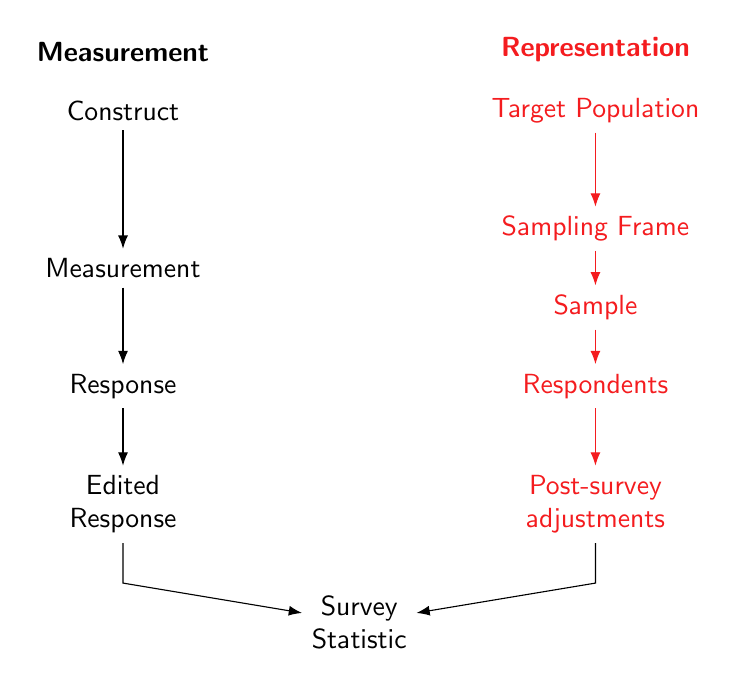
\begin{tikzpicture}[
meas/.style = {
	align=center
	},
rep/.style = {
	align=center,
	aured
	},
measArr/.style = {
	-Latex
	},
repArr/.style = {
	-Latex,
	aured
	}
]

\node [meas, above] at (3,0) {\textbf{Measurement}};
\node [rep, above] at (9,0) {\textbf{Representation}};

% MEASUREMENT NODES
\node [meas] (measA) at (3,-.5) {Construct};
\node [meas] (measB) at (3,-2.5) {Measurement};
\node [meas] (measC) at (3,-4) {Response};
\node [meas] (measD) at (3,-5.5) {Edited\\Response};
\node (stat) [align=center] at (6,-7) {Survey\\Statistic};

% REPRESENTATION NODES
\node [rep] (repA) at (9,-.5) {Target Population};
\node [rep] (repB) at (9,-2) {Sampling Frame};
\node [rep] (repC) at (9,-3) {Sample};
\node [rep] (repD) at (9,-4) {Respondents};
\node [rep] (repE) at (9,-5.5) {Post-survey\\adjustments};

% PATHS
\path [measArr] (measA) edge (measB) (measB) edge (measC) (measC) edge (measD);
\draw [-Latex] (measD) to (3,-6.5) to (stat);
\path [repArr]  (repA) edge (repB) (repB) edge (repC) (repC) edge (repD) (repD) edge (repE);
\draw [-Latex] (repE) to (9,-6.5) to (stat);
\end{tikzpicture}

\end{document}